High-performance computing (HPC) applications must exploit parallelism
in order to take advantage of all of the hardware resources of
modern multicore nodes, potentially with some form of heterogeneity
(e.g. specialized coprocessors).
Obviously, there are a number of ways to map algorithmic concurrency
to hardware parallelism, which on general purpose processors rely
upon either multithreading or multiprocessing, which are different
from the user perspective but very similar from the perspective of
the operating system and hardware.
OpenMP is the most popular programming model for multithreading in HPC,
although it is far from the only one.
Other portable threading models that may be used in HPC include
POSIX threads,
Intel\regtm{} Threading Building Blocks (TBB)~\cite{pheatt2008intel},
%\footnote{TBB is build on top
%of POSIX\othertm{} threads (at least on Linux\othertm{} systems), and is portable to
%processors from AMD\othertm, ARM\othertm, IBM\othertm, Intel and other vendors.},
ISO\othertm{} C11 and C++ threads, and
OpenCL\othertm.

In addition to the aforementioned explicit use of threads in HPC applications,
threads may be used implicitly in language concurrent features such as
ISO C++11 \texttt{std::async} and \texttt{std::future},
ISO Fortran 2008 \texttt{DO CONCURRENT} and coarray images.
%\footnote{
%The Fortran standard does not specify how coarray images are implemented,
%but it almost certainly involves either OS threads or OS processes.}.
Both compute and runtime libraries may use threads;
compute libraries that implement BLAS, LAPACK or FFT functions
currently use at least four different threading models internally and
runtime libraries such as MPI may spawn threads to implement asynchronous progress.
Finally, in addition to multiple forms of threads, there may be multiple
processes executing the application code on the node, the most obvious example
of which is when MPI is used.  However, for purposes of this paper, we will 
consider multiprocessing differently from multiprocessing,
due to their similarities as it pertains to interoperability problems.

In cases where OpenMP is coexisting with at least one other threading model,
we can identify at least three classes of scenarios in which to consider
interoperability: Phased, Concurrent and Nested.
These are illustrated in Figure~\ref{fig:interop-motif}.
Threaded applications that call libraries that use a different threading model
are a good example of the Phased motif.
The thread(s) inside of e.g. an MPI library used by an OpenMP application
matches with the Concurrent motif.
Nested can be either OpenMP threads calling application or library
functions that use another threading model, or the other way around.
Of course, in all cases, the coexistence may not be as regular as
the picture describes, but these simple cases are sufficient to reveal
the challenges of interoperating multiple threading models.
\begin{figure}[htb]
\centering
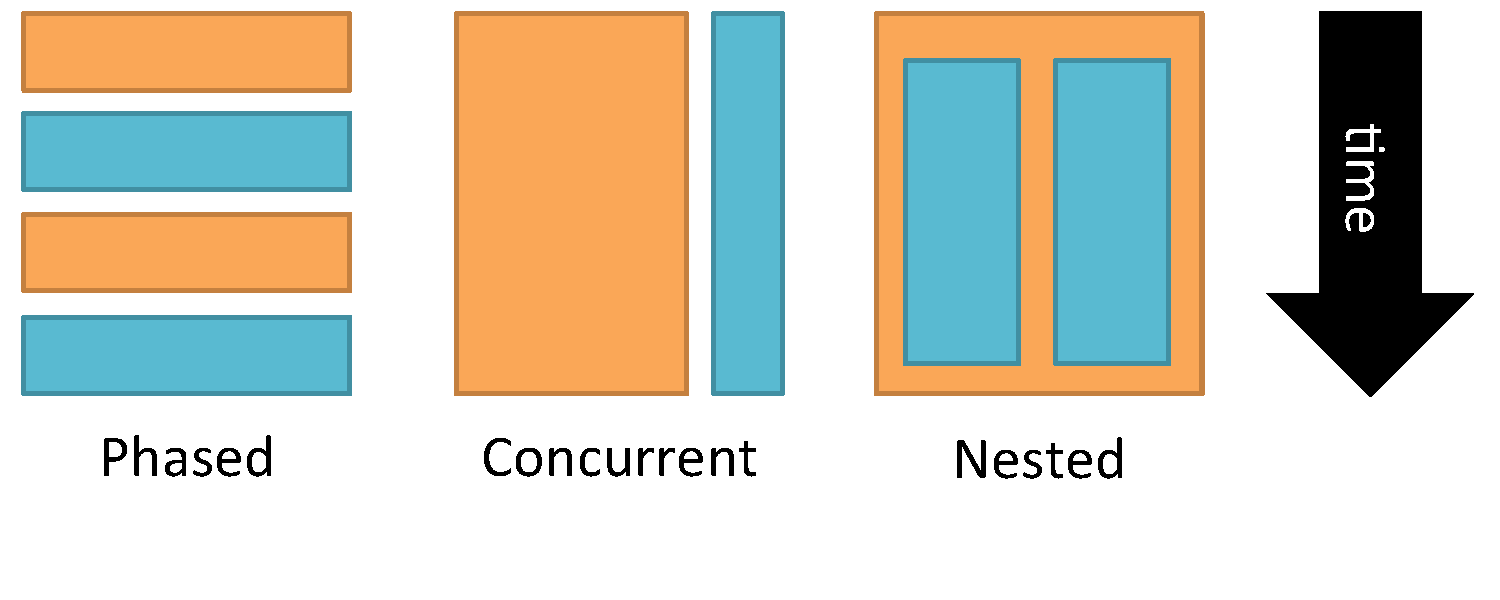
\includegraphics[width=0.5\textwidth]{images/interop-motifs}
\caption{Pictoral description of Phased, Concurrent and Nested
motifs where two threading models must interoperate.
\label{fig:interop-motif}
}
\end{figure}

\begin{comment}

Applications are using multiple threading models.
Common ones include OpenMP\othertm, POSIX threads, TBB, OpenCL\othertm.
Now that ISO\othertm C11 and C++11 both have threads, and C++11 has
std::async, std::future, etc., programmers have many
ways to create threads in a program.

Libraries are written independent of applications, will use what is best
aligned with their design, or which is most interoperable (like OS threads).
Some libraries may need to be called from threaded region, but often not.

Runtimes often use threads, but in a very different way from applications.
Example of MPI or PGAS runtime with communication helper threads.
OpenMP task cannot be used here since cannot use outside of parallel region.
Runtime threads must interact with OS in deep way, so OS threads make sense.

Primary problem is oversubscription of hardware threads, which causes
major performance issues, particularly on HPC-oriented lightweight operating systems
(e.g. IBM Blue Gene CNK).

Secondary problem of affinity.
Even if software threads do not oversubscribe hardware threads,
are software threads running on the right set of resources at the right time.
Best performance often achieved with affinity binding to specific resources,
which creates oversubscription for a specific resource, even if not globally.

Three approaches:
(1) explicit thread creation
(2) wait policy
(3) quiesce

(1) assumes every client of threads buys into it, which is not going to happen,
even though the API is aligned with POSIX/Windows/Solaris thread APIs.
Example of clone() for Cray XT Seastar/Portals3 in ARMCI.
However, may be particularly useful for HPC systems, where full-blown POSIX
threads are too much, and simple OS threading model is sufficient
(IBM Blue Gene is a good example of this).
MPI libraries support POSIX/Solaris/Windows threads already -- would
not be difficult to support OpenMP abstraction for OS threads,
at least in HPC environments.

(2) wait policy causes threads to back off and potentially go to
sleep while other threads are running.
However, these sleeping threads are parked in the kernel and may
still cause some OS scheduling overhead, if not sufficiently passive.
How long before threads back off completely?
Will this always happen before other threading model is running?
Do sleeping threads have affinity consequences?  If pinned, possibly.
Even Intel monitor-mwait consumes the hardware thread
(Blue Gene interrupt/wakeup unit does not).
Aggressive wait policy is great for interop but hurts latency.
Have to pull all threads out of sleep for new parallel region.
Forces application to pay tax on every fork-join when not required.
Some OpenMP codes do lots of fork-join, and it is likely optimal to
spin-wait in serial regions, at least for a short period, to ensure
the lowest latency of parallel region creation.

(3) is heavy hammer but allows for bulk sync phased interop, which
is especially useful for libraries.
Likely more expensive than most aggressive wait policy, but the cost
of recreation is only paid after when quiesce is used explicitly, when needed.
In some cases, quiesce may just invoke deep sleep, not actually destroy
thread pool, but this still permits the threads to use low-latency
wait policy between join and fork.

\end{comment}

\begin{comment}
Large-scale parallel applications are typically developed using multiple parallel programming models in 
a hybrid fashion, e.g. MPI+OpenMP, and using one or mulitple prebuilt scientific and/or platform-specific libraries such as Intel Math Kernel Library (MKL)~\cite{wang2014intel}.
Each of these programming models and libraries often has its own runtime library to handle scheduling of work units and management of computational
and data movement tasks. 
There have been challenging issues for using these models in one application, including 
compatibility issues for compiling and linking, oversubscription of resources at runtime, and the naming conflicts that 
programmers have to create workaround wrappers to deal with.

This paper proposes solutions to the interoperability and composability challenges faced by the OpenMP programming interface, includling those
between multiple OpenMP implementations and/or multiple OpenMP runtime instances of the same implementation, OpenMP 
with native threads (Pthreads and Windows Native threads), OpenMP with other threading languages and libraries such 
as C++11, TBB and Cilkplus, and OpenMP with inter-node programming models such as MPI and PGAS. We 
think the similar challenges exist in other threading based libraries and language implementations, and believe
the solutions we provided  will work for them too.  

Interoperability and composability are closely related, while the interoperability sounds to improve the interactions between multiple models
while composability is meant to improve the modular use of OpenMP with itself and other models. One is from the aspect of system while 
the other is more concerned with software engineering. Both should be considered when developing solutions. 

For parallel programming languages and libraries, most implementations rely on system native threading (Pthreads or Windows Native threads) 
mechanisms to acquires system resources. Each implementation of the same or different programming models has their own mechanism for scheduling
user-level tasks and operations, which is the core part of a runtime system. 
The interoperability challenges are then concerned with how much we want two or more 
runtime instances (for the same or different high-level programming interfaces) to interact with other other for computational resource sharing
and data movement. Thus solutions to these challenges are more in the scope of runtime implementation, than in the level of programming
interfaces and compiler transformations. 
\TODO{I guess there might be language features enabling interoperability. Also are runtime library interfaces part of programming interfaces??}

\end{comment}

\REM{
\subsection{What is an OpenMP?}
OpenMP is an implementation model to support the implementation of parallel algorithms. It is primarily designed for shared memory multiprocessors. The goal of OpenMP is to provide a standard and portable API for writing shared memory parallel programs~\cite{dagum1998openmp}. 

OpenMP takes a directive-based approach for supporting parallelism. It consists of a set of directives that may be embedded within a program written in a base language such as Fortran, C, or C++. There are two compelling benefits of a directive-based approach that led to this choice: The first is that this approach allows the same code base to be used for development on both single-processor and multiprocessor platforms; on the former, the directives are simply treated as comments and ignored by the language translator, leading to correct serial execution. The second related benefit is that it allows an incremental approach to parallelism—starting from a sequential program, the programmer can embellish the same existing program with directives that express parallel execution. These directives may be offered within any base language (within the C/C++ languages, directives are referred to as “pragmas”). In addition to directives, OpenMP also includes a small set of runtime library routines and environment variables. These are typically used to examine and modify the execution parameters. The language extensions in OpenMP fall into one of three categories: control structures for expressing parallelism, data environment constructs for communicating between threads, and synchronization constructs for coordinating the execution of multiple threads~\cite{chandra2001parallel}.
\subsection{How does OpenMP work?}
OpenMP uses a fork/join execution model. OpenMP provides two kinds of constructs for controlling parallelism. First, it provides a directive to create multiple threads of execution that execute concurrently with each other. The only instance of this is the parallel directive. Second, OpenMP provides constructs to divide work among an existing set of parallel threads. An instance of this is the do directive. 

An OpenMP program always begins with a single thread of control that has associated with it an execution context or data environment. This initial thread of control is referred to as the master thread. When the master thread encounters a parallel construct, new threads of execution are created along with an execution context for each thread. Each thread has its own stack within its execution context. The execution context for a thread is the data address space containing all the variables specified in the program. Multiple OpenMP threads communicate with each other through ordinary reads and writes to shared variables.
\subsection{OpenMP Runtime Library}
The OpenMP API runtime library routines are external procedures. The return values of these routines are of default kind, unless otherwise specified. Runtime library provides interface to the compiler. The runtime interface is based on the idea that the compiler ``outlines`` code that is to run in parallel into separate functions that can then be invoked in multiple threads. OpenMP provides several runtime library routines to assist you in managing your program in parallel mode. Many of these runtime library routines have corresponding environment variables that can be set as defaults. The runtime library routines enable you to dynamically change these factors to assist in controlling your program. In all cases, a call to a runtime library routine overrides any corresponding environment variable. 

Generally, we can analyze the architecture into two perspectives: the parallelization regions and the data.
\begin{enumerate}
	\item Region perspective.
	We use “parallel” to automatically create multi-threads. And each thread will be executed without order. However, we can use ordered clause to guarantee the code be executed in sequence. There are different types of parallel regions:
	\begin{itemize}
		\item Section means the task is assigned to each thread.
		\item Single means the task is assigned to a random thread.
		\item Master means the task is executed in the master thread.
	\end{itemize}
	For the default parallel regions, we can use “schedule” to design a way to assign tasks to different threads. Generally, we can implement this assignment in three ways:
	\begin{itemize}
		\item Static: equally assign them to n threads.
		\item Dynamic: assign them to the idle thread only.
		\item Guided: implement the dynamic assignment reductively.
	\end{itemize}
	\item Data perspective.
	We have two kinds of variables. Variables that are defined before parallel region are shared among every thread, while those defined in parallel regions can be only accessed by certain threads. We use “threadprivate” to change those shared variables into a private one for each thread. This is done by generating a new private variable for every single thread. For those shared variables, we must pay attention to the data race problem, which defined as two different memory operations are trying to use a same variable, and different execution order may lead to different results. To solve this problem, we can use “critical” or “atomic” directive to guarantee that the data can be only accessed by one thread at a time. We can also set “barriers” to make sure all threads have been executed before starting any new threads. Sometimes the update of certain variables are stored only in registers, we can use “flush” to directly write the data back to memory to make sure that other threads will use the data that already been updated.
\end{enumerate}
}
